\documentclass[11pt,a4paper]{article} 

\usepackage[dutch]{babel} %needs to specified for minutes package (else it will be in German)
\usepackage{a4wide}%For a wider spacing of the text (smaller left/right margin)
\usepackage{graphicx}
\usepackage{setspace}
\usepackage{minutes}

\pagestyle{plain}
\usepackage{todositemized}
%more memmorable commands to make the checked and crossed symbols





%%%%%%%%%%%%%%%%%%%%%%%%%%%%%%%%%%%%%%%%%%%%%%%%%%%%%%%%%%%%%%%%%%%%%%%%%%%%%%%
%
% Important: This template compiles without errors
% always check errors, also the yellow ones, even if you get a PDF
%
%%%%%%%%%%%%%%%%%%%%%%%%%%%%%%%%%%%%%%%%%%%%%%%%%%%%%%%%%%%%%%%%%%%%%%%%%%%%%%%%





\newpage



\usepackage[dutch]{babel} %needs to specified for minutes package (else it will be in German)
\usepackage{a4wide}%For a wider spacing of the text (smaller left/right margin)

\usepackage{setspace}
\usepackage{minutes}

\pagestyle{plain}
\usepackage{todositemized}
%more memmorable commands to make the checked and crossed symbols





%%%%%%%%%%%%%%%%%%%%%%%%%%%%%%%%%%%%%%%%%%%%%%%%%%%%%%%%%%%%%%%%%%%%%%%%%%%%%%%
%
% Important: This template compiles without errors
% always check errors, also the yellow ones, even if you get a PDF
%
%%%%%%%%%%%%%%%%%%%%%%%%%%%%%%%%%%%%%%%%%%%%%%%%%%%%%%%%%%%%%%%%%%%%%%%%%%%%%%%%



\begin{document}

\begin{Minutes}{Notulen Poject Natuurkunde, groepje 24}


%Add relevant date, time and location here
\minutesdate{17-06-2023} %Write the date of when you finish the minutes
\starttime{11:00}
\endtime{}
\location{}

%Add relevant names here
\participant{Tom, Noah} 
\minutetaker{Tom}

% \moderation{Niemand} 
%In case people are not present


\maketitle



\newpage


\section{Mededelingen} 
Vandaag hebben we vooral aan het schrijven van code besteed. Als eerste heeft Tom een code gemaakt die een differentiaalvergelijking kan oplossen uit een artikel. Daarna heeft Tom wat tijd aan de poster besteed terwijl Noah zijn code voor het bepalen van $E^*$ aan het verbeteren. Toen dat was gelukt hebben Tom en Noah de resultaten van $G'$ t.o.v $E^*$ geplot op verzoek van Antoine. De supervisor had verwacht dat hij lineair zou lopen maar hij loopt exponentieel. Daarna heeft Noah nog wat verbanden tussen formules getrokken terwijl Tom verder aan de poster werkte. Richting het einde van de dag heeft Antoine het nog gehad over een mogelijke fit voor $G'$ die we kunnen gebruiken voor het geval we niet meer op tijd de data op -30 graden kunnen meten. Daarna heeft Antoine nog een keer goed uitgelegd wat het doel van het onderzoek was zodat we het goed kunnen gaan zetten op de poster. Tom en Noah hebben als laatste nog allebei gewerkt aan het maken van een mooi grafiek voor op de poster. Talha is absent in verband met overleden familielid. 


\section{Wat moeten we nu doen/bespreken?}
Hopelijk de metingen op -30 graden en anders dus een fit, en aan de poster verder werken.

\section{Figuren}
\begin{figure}[h]
    \centering
    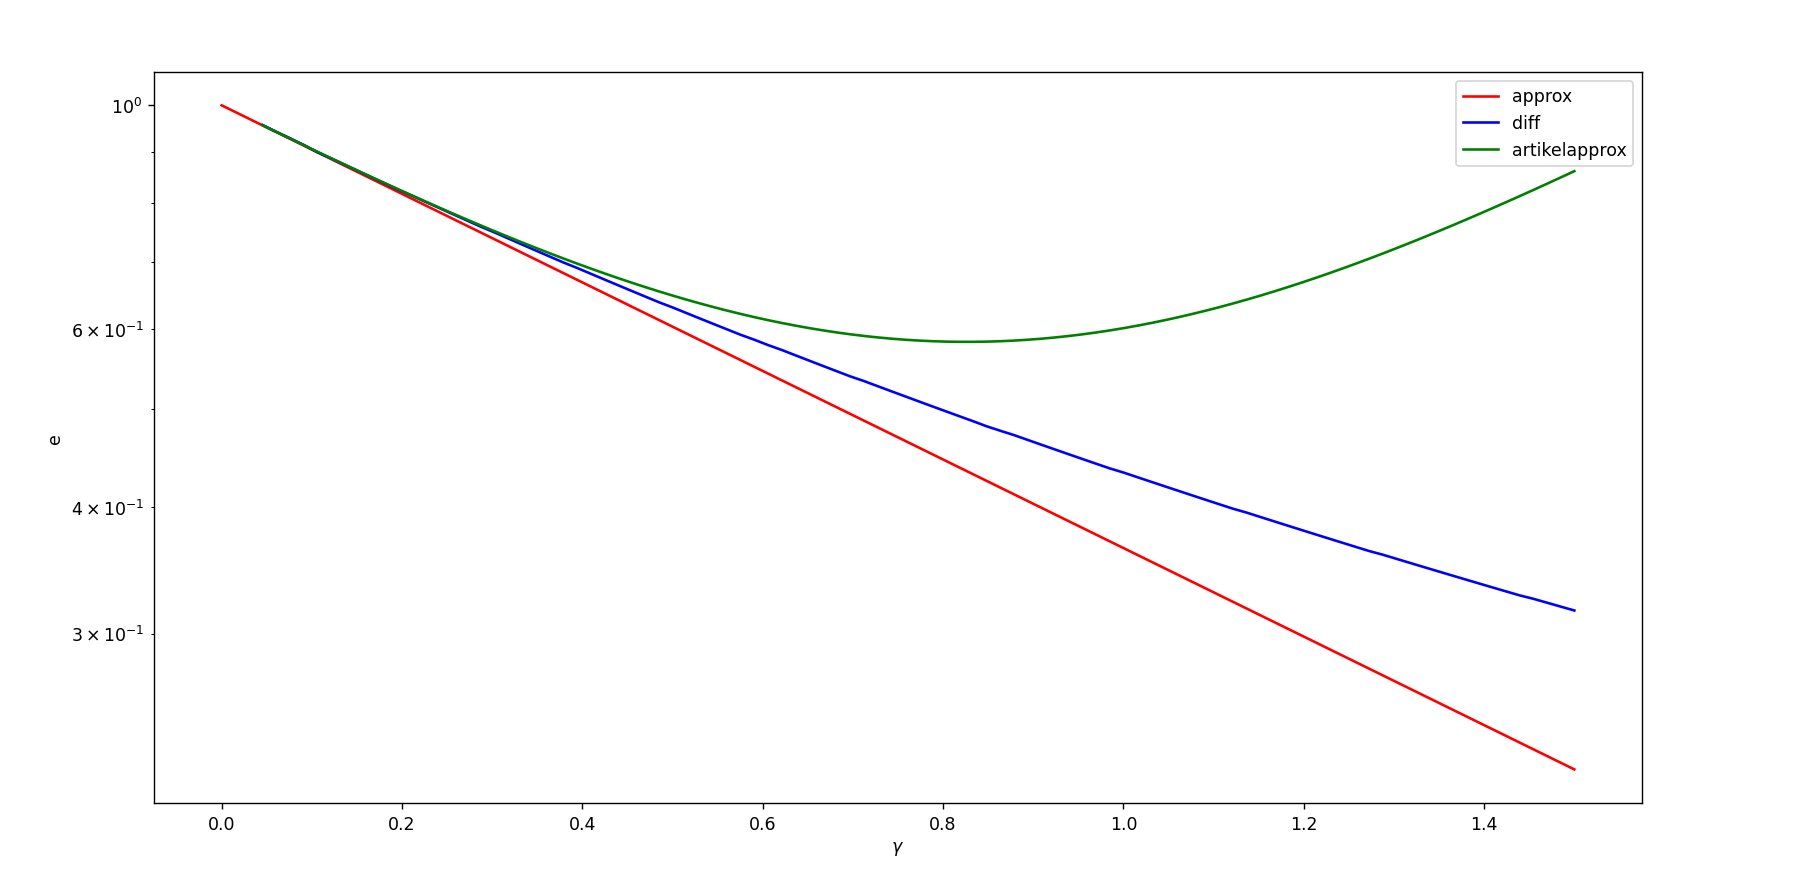
\includegraphics[width=0.5\linewidth]{Schermafbeelding 2025-06-20 103839.png}
    \caption{Dit is een grafiek van een functie die de differentiaalvergelijking beschrijft binnen een bepaald marge. We hebben de approx functie gebruikt omdat deze het makkelijkst te gebruiken is en ongeveer net zo accuraat is als de functie uit het artikel (Hertz beyond belief)}
    \label{fig:enter-label}
\end{figure}

\end{Minutes}
\end{document}




\section{Oude actiepunten}
Zijn er niet.

\section{Wat moeten we nu doen/bespreken?}

\subsection{Wie wil en kan wat?}

\task{talha}{checklist}

\subsection{Communicatie}


\subsection{Beschikbaarheid}


\section{Checklist uit de Powerpoint}



\section{Overige punten}
We wachten even morgen af, als we met Antoine spreken.

\section{Nieuwe actiepunten}
\listoftasks
\section{Volgende vergadering}
De volgende bijeenkomst is morgen met de begeleider, bij het fancy koffiezet apparaat bij D.

\section{Afsluiting vergadering}
De vergadering is om 12:49 gesloten.


\end{Minutes}
\end{document}